\section{Introduction to Reinforcement Learning}
Learning from interaction is an idea that is at the basis of nearly all theories of learning and intelligence, among which we find reinforcement learning.

Reinforcement learning is learning what to do and how to map situations to actions, so as to maximize a numerical reward (it is goal-directed learning from interaction). The learner is not told which actions to take, but instead it must discover which actions yield the most reward by trying them. In the most interesting and challenging cases, actions may affect not only the immediate reward but also the next situation and, through that, all subsequent rewards. These two characteristics (trial-and-error search and delayed reward) are the two most important distinguishing features of reinforcement learning.

We will now introduce finite Markov decision processes, a mathematical framework that we are going to use.

\subsection{Finite Markov Decision Processes}
Markov Decision Processes (MDPs) are a mathematically idealized formulation of reinforcement learning for which precise theoretical statements can be made. They provide a mathematical framework for modeling decision making in situations where outcomes are partly random and partly under the control of a decision maker\footnote{See \url{https://en.wikipedia.org/wiki/Markov_decision_process}}.

At each time step $t$, the process is in some state $s$, and the decision maker may choose an action $a$ that is available in state $s$. The process responds at the next time step by randomly moving into a new state $s'$, and giving the decision maker a corresponding reward $R_a(s,s')$. The probability that the process moves into its new state $s'$ is influenced by the chosen action. Specifically, it is given by the state transition function $P_a(s,s')$. Thus, the next state $s'$ depends on the current state $s$ and the decision maker's action $a$. But \textbf{given $s$ and $a$, it is conditionally independent of all previous states and actions}; in other words, the state transitions of an MDP satisfy the Markov property \textit{(memoryless property of a stochastic process)}.

\begin{figure}[hbt]
    \centering
    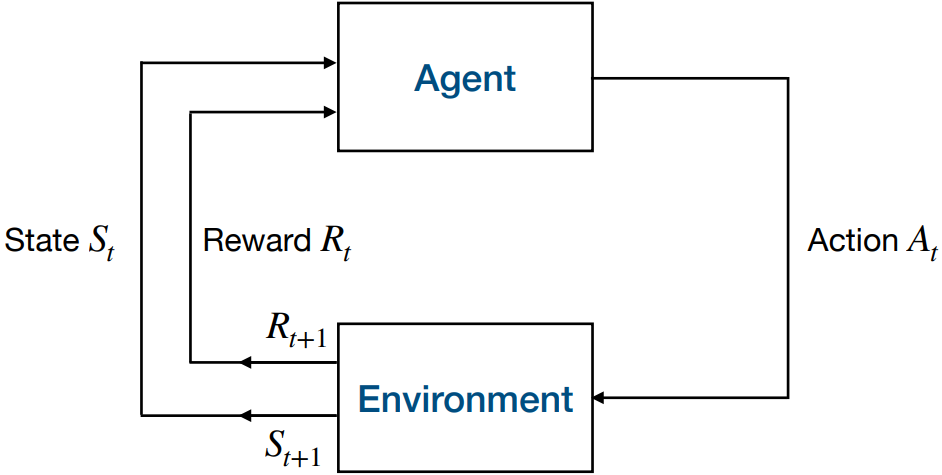
\includegraphics[width=\textwidth]{Images/Chapter 2/mdp.png}
    \caption{Schema of a Markov Decision Process.}
    \label{fig:ch2-mdp}
\end{figure}

\subsection{Rewards and expected returns}
Informally, the agent’s goal is to maximize the \textbf{total amount} of rewards it receives (note how the agent should not maximize the immediate reward, but the cumulative reward). We can formalize this with the \textbf{``reward hypothesis''}: \textit{``That all of what we mean by goals and purposes can be well thought of as the maximization of the expected value of the cumulative sum of a received scalar signal (called reward)''}.

We will now try to conceptualize the idea of \textbf{cumulative rewards} more formally by means of the notion of \textbf{expected return} $G_t$. To do so, we first need to distinguish between two cases:
\begin{itemize}
    \item \textbf{Episodic tasks}, in which we can identify a final step of the sequence of rewards (i.e., in which the interaction between the agent and the environment can be broken into sub-sequences called \textbf{episodes}, such as playing a game, repeated tasks, etc.). Each episode ends in a terminal state after $T$ steps, followed by a reset to a standard starting state or to a sample of a distribution of starting states (the next episode will be completely independent from the previous one).
    \item \textbf{Continuous tasks}, in which the agent-environment interaction does not break naturally into identifiable episodes, but goes on continually without limit (e.g., an ongoing monitoring of a process).
\end{itemize}

The expected return $G_t$ associated to the selection of an action $A_t$, assuming that the agent receives over time a sequence of rewards $R_{t+1}, R_{t+2}, R_{t+3}, ...$ is defined as:
\begin{itemize}
    \item The sum of the future rewards \textbf{in the case of episodic tasks}:
    \begin{equation}
        G_t \doteq R_{t+1} + R_{t+2} + R_{t+3} + ... + R_t
        \label{eq:ch2-expectedreturn-episodic}
    \end{equation}
    \item The weighted sum of the future rewards \textbf{in the case of continuing tasks}:
    \begin{equation}
        G_t \doteq R_{t+1} + \gamma R_{t+2} + \gamma^2 R_{t+3} + ... = \sum_{k=0}^{\infty} \gamma^k R_{t+k+1}
        \label{eq:ch2-expectedreturn-continuous}
    \end{equation}
\end{itemize}

Where $\gamma$ is the \textbf{discount rate}, with $0 \le \gamma \le 1$. The discount rate is used to give more importance to the rewards that are closer to us in time; this is particularly useful in dynamic environments. The definition of expected return that we used for episodic tasks would in fact be problematic for continuing tasks: the expected return at the time of termination $T$ would be equal to $\infty$ in some cases, such as when the reward is equal to $1$ at each time step. The discount rate determines the ``present value of future rewards'' (how much future rewards mean to us at the current time): a reward received $k$ time steps in the future is worth $\gamma^{k-1}$ of what it would be worth if it were received immediately.

Returns at successive time steps are related to each other as follows:
\begin{equation*}
    \begin{split}
        G_t & \doteq R_{t+1} + \gamma R_{t+2} + \gamma^2 R_{t+3} + \gamma^3 R_{t+4} + ... \\
        & = R_{t+1} + \gamma \left( R_{t+2} + \gamma R_{t+3} + \gamma^2 R_{t+4} + ... \right) \\
        & = R_{t+1} + \gamma G_{t+1} \\
    \end{split}
\end{equation*}

\subsection{Policies and value functions}
Almost all reinforcement learning algorithms involve estimating value functions, i.e., functions of states (or of state-action pairs) that estimate how good it is for the agent to be in a given state (or how good it is to perform a given action in a given state). The notion of ``how good'' here is defined in terms of future rewards that can be expected, or, to be precise, in terms of expected return.

A \textbf{policy} is used to model how the agent will behave based on the previous experience and the rewards (and, consequently, the expected returns) an agent received in the past. Formally, a policy is a mapping from states to probabilities of each possible action (the probability of taking a certain action in a certain state). If the agent is following the policy $\pi$ at time $t$, then $\pi (a \vert s)$ is the probability that $A_t=a$ if $S_t=s$.

\textbf{The value function of a state s under a policy $\pi$}, denoted $v_\pi (s)$, is the expected return when starting in $s$ and following $\pi$ thereafter (the expected return I can have in the future state, considering all the actions I might take from there). For Markov Decision Processes, we can define \textbf{the state-value function} $v_\pi$ for the policy $\pi$ formally as:
\begin{equation}
    v_s \doteq \mathbb{E}_\pi \left[ G_t \vert S_t = s \right] = \mathbb{E}_\pi \left[ \sum_{k=0}^{\infty}  \gamma^k R_{t+k+1} \middle\vert S_t = s, A_t = a \right] \quad \forall s \in \mathcal{S}
    \label{eq:ch2-statevaluefunction}
\end{equation}

Where $\mathbb{E}_\pi [\cdot]$ denotes the expected value of a random variable given that the agent follows $\pi$ and $t$ is any time step. Note that the value of the terminal state, if any, is always $0$. The formula above denotes a weighted average of the expected value (it is averaged because the values depend on the probability of a certain action being taken, which is a fraction).

Similar to what we just did, we can define \textbf{the action-value function}, i.e., the value of taking an action $a$ in the state $s$ under a policy $\pi$, denoted $q_\pi (s,a)$, as the expected return starting from $s$, taking the action $a$, and following the policy $\pi$ thereafter:
\begin{equation}
    q_\pi(s,a) \doteq \mathbb{E}_\pi \left[ G_t \vert S_t = s, A_t = a \right] = \mathbb{E}_\pi \left[ \sum_{k=0}^{\infty} \gamma^k R_{t+k+1} \middle\vert S_t = s, A_t = a \right]
    \label{eq:ch2-actionvaluefunction}
\end{equation}

\subsection{Choosing the rewards}
When we model a real system as a reinforcement learning problem, the most difficult task is selecting the right rewards. Typically, we use negative values for actions that do not help us in reaching our goal, and positive if they do (it is also possible using 0 as a value for actions that do not help us). An alternative is to set the values of rewards to a negative number until we reach our goal (using 0 as the value when we reach it).

When choosing the rewards, it is very important that \textbf{we should not ``reward'' the intermediate steps or the single actions}. The agent, in fact, always learns to maximize its reward. If we want it to do something for us, we must provide rewards to it in such a way that in maximizing them the agent will also achieve our goals. It is thus critical that the rewards we set up truly indicate what we want accomplished. If we were to give importance to certain sub-goals, the agent might find a way to achieve them without achieving the real goal (e.g., taking the opponent's pieces while playing chess but losing the game). Note that the reward signal is our way of communicating to the agent \textit{what} we want achieved, not \textit{how} a better place for imparting this kind of prior knowledge would be the initial policy or the initial value function.